\documentclass[tikz,border=3mm,multi=tikzpicture]{standalone}
\usepackage[utf8]{inputenc}
\usepackage[T1]{fontenc}
\usepackage{helvet}
\renewcommand{\familydefault}{\sfdefault}
\usepackage{tikz}
\usetikzlibrary{arrows.meta,positioning,circuits.ee.IEC}
\begin{document}

\tikzset{every node/.append style={font=\sffamily\small}}

% TikZ 1
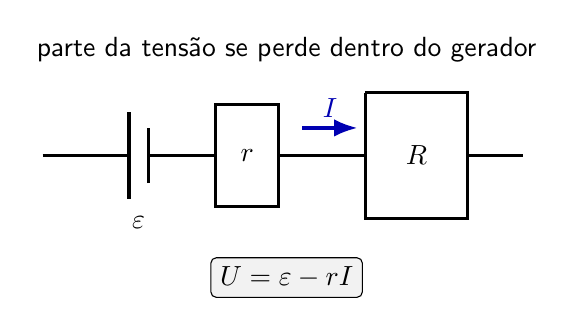
\begin{tikzpicture}[>=Latex]
  \draw[very thick] (0,0) -- (1.1,0);
  \draw[very thick] (1.1,-0.55) -- (1.1,0.55);
  \draw[very thick] (1.35,-0.35) -- (1.35,0.35);
  \node[below] at (1.22,-0.65) {$\varepsilon$};
  \draw[very thick] (1.35,0) -- (2.2,0);
  \draw[very thick] (2.2,0) -- (2.2,0.65) -- (3.0,0.65) -- (3.0,-0.65) -- (2.2,-0.65) -- (2.2,0);
  \node at (2.6,0) {$r$};
  \draw[very thick] (3.0,0) -- (4.1,0);
  \draw[very thick] (4.1,0.8) -- (4.1,-0.8) -- (5.4,-0.8) -- (5.4,0.8) -- (4.1,0.8);
  \node at (4.75,0) {$R$};
  \draw[very thick] (5.4,0) -- (6.1,0);
  \draw[very thick,->,blue!70!black] (3.3,0.35) -- (4.0,0.35) node[midway,above] {$I$};
  \node[draw,rounded corners=2pt,fill=gray!10,align=center] at (3.1,-1.55)
    {$U=\varepsilon-rI$};
  \node[align=center] at (3.1,1.35) {parte da tensão se perde dentro do gerador};
\end{tikzpicture}

% TikZ 2
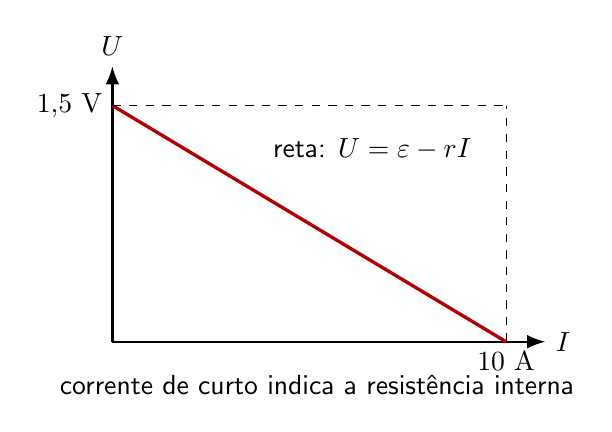
\begin{tikzpicture}[x=1cm,y=1cm,>=Latex]
  \draw[->,thick] (0,0) -- (5.5,0) node[right] {$I$};
  \draw[->,thick] (0,0) -- (0,3.5) node[above] {$U$};
  \draw[very thick,red!70!black] (0,3) -- (5,0);
  \node[left] at (0,3) {$1{,}5\ \mathrm{V}$};
  \node[below] at (5,0) {$10\ \mathrm{A}$};
  \draw[dashed] (0,3) -- (5,3);
  \draw[dashed] (5,0) -- (5,3);
  \node[align=center] at (3.3,2.45) {reta: $U=\varepsilon-rI$};
  \node[align=center] at (2.6,-0.55) {corrente de curto indica a resistência interna};
\end{tikzpicture}

\end{document}
